% MSc Dissertation on pattern expression in Ovarian Cancer

\documentclass[tikz, 12pt,a4paper,oneside,fleqn]{article}
\usepackage[margin=2cm]{geometry}
\usepackage[utf8]{inputenc}
\usepackage{amsmath}
\usepackage{amsfonts}
\usepackage{amssymb}
\usepackage{fancyvrb}
\usepackage{setspace}
\usepackage{enumitem}
\setlist[description]{leftmargin=\parindent,labelindent=\parindent}

\usepackage{caption}
\captionsetup[figure]{labelfont=bf,format=hang,font={stretch=1.2, small}}
\captionsetup[table]{labelfont=bf,format=hang,font={stretch=1.2, small}}


\usepackage[linewidth=1pt]{mdframed}


\usepackage{graphicx}


\graphicspath{{/home/ipoole/Documents/gitrepos/MScDissertation/images/}}  % trailin '/' is required!


\newcommand{\plotspath}[1]{{/home/ipoole/Documents/gitrepos/HgsocTromics/Plots/#1}}


\usepackage{hyperref}
\usepackage{subfig}
\usepackage{booktabs}  % Needed for pandas to_latex() output
\usetikzlibrary{positioning}


\newcommand{\etal}{{\em et al\/}}
\newcommand{\comment}[1]{\marginpar{{\tiny\singlespacing #1 \par}}}

\linespread{1.5}
% This sets Arial font (bit ugly!)
\usepackage{helvet}
\renewcommand{\familydefault}{\sfdefault}

%\usepackage{titlesec}
%\titleformat{\subsubsection}
%   {\itshape\normalsize}{\thesubsubsection}{1em}{}


%%%%%%%%%%%%%%%%%%%%%%%%%%%%%%% SUBMISSION PAGE %%%%%%%%%%%%%%%%%%%%%%%%%%%%

\thispagestyle{empty}

\title{Phylogenetic study of Asgard Archaea}
\author{}

\begin{document}

%%%%%% Assesment Title Page
\begin{center}

\includegraphics[scale=0.3]{images/UoE_SBO_logo.png}
\end{center}

\vspace{0.3in}

\begin{mdframed}
\begin{center}
\huge
\vspace{0.3in}
\bf
Disentangling patterns of gene expression in high grade serous ovarian cancer
\vspace{0.2in}
\end{center}
\vspace{0.2in}
\end{mdframed}

\vspace{0.3in}

\begin{mdframed}
\begin{center}
\large
\vspace{0.2in}
Student Exam Number: \bf{B156476}
\vspace{0.2in}
\end{center}
\end{mdframed}

\vspace{0.3in}

\begin{mdframed}
\begin{center}
\large
\vspace{0.2in}
In partial fulfilment of the requirement for the Degree of
Master of Science in Systems and Synthetic Biology at the
University of Edinburgh,
2019 / 2020
\vspace{0.2in}
\end{center}
\end{mdframed}

\vspace{0.3in}

\begin{mdframed}
\begin{center}
\large
\vspace{0.2in}

Disssertation Supervisor:  Dr. Ailith Ewing
\vspace{0.2in}
\end{center}
\end{mdframed}

\newpage
\setcounter{page}{1}
%\pagestyle{headings}

%%%%%%%%%%%%%%%%%%%%%%%%%%% Start of report for real %%%%%%%%%%%%%%%%%%%


\section{Introduction}

Research questions:  
\begin{enumerate}
\item What are the known patterns of gene expression in high-grade serous ovarian cancer?
\item How can blind-source separation techniques such as independent component analysis and non-negative matrix factorization be applied to transcrptomics studies?
\item How can biological databases be used to link genes into oncogenesis pathways?
\end{enumerate}

\subsection{Matrix factorization methods}
\label{sec-matrix-factorization-intro}

A good introduction is found in ref \cite{Stein-OBrien2018} matrix factorization (MF) methods are discussed as a means of extraction the low dimensional structure from a high dimensional ``-omics" datasets, with gene expression analysis being the prime example.  
Conventionally, transcriptomics expression arrays are oriented with genes (or transcripts) as rows, and samples (e.g. patients) in columns.   
A typical expression array might have in the order of tens of thousands of rows and hundreds of columns.  
MF methods reduces this large $M \times N$ (genes $\times$ samples) matrix into two two smaller matrices.
In the terminology of Stein-O'Brien \etal\ these are the $M \times K$ \emph{pattern matrix} and the $K \times N$ \emph{amplitude matrix}.  $K$ is typically small of the order 10, and refers to the number of extracted \emph{factors} (or components). 

\begin{figure}[ht]
\def\M{2.2cm}
\def\N{1.3cm}
\def\K{0.3cm}
\def\fudge{-0.8mm}
\centering

\subfloat[Optimising independence of Meta\underline{genes}]{
\begin{tikzpicture}[node distance = 0.25cm]
	\node (X) [draw, fill=green, minimum height=\M, minimum width=\N] {\large X};
	\node [right=of X] (eq) {\large $\approx$};
	\node [right=of eq] (S) [draw, fill=yellow, minimum width=\K, minimum height=\M] {\large S};
	\node [right=of S] (times) {\LARGE$\times$};
	\node [right=of times] (A) [draw, fill=cyan, minimum width=\N, minimum height=\K] {\large A};
	
	\node [below=\fudge of X] {\tiny{$N$ Samples}};
	\node [left=\fudge of X] {\rotatebox{90}{\tiny{$M$ Genes}}};
	\node [below=of X, text width=2cm, align=center] {\small Expression matrix};
	
	\node [below=\fudge of S] {\tiny{$K$ Metagenes}};
	\node [left=\fudge of S] {\rotatebox{90}{\tiny{$M$ Genes}}};
	\node [below=of S, text width=2cm, align=center] {\small Metagenes};
	
	\node [below=\fudge of A] {\tiny{$N$ Samples}};
	\node [left=\fudge of A] {\tiny{$K$}};
	\node [below=of A, text width=2cm, align=center] {\small Metasamples};
\end{tikzpicture}}

\subfloat[Optimising independence of Meta\underline{samples}]{
\begin{tikzpicture}[node distance = 0.25cm]
	\node (X) [draw, fill=green, minimum height=\N, minimum width=\M] {\large X};
	\node [right=of X] (eq) {\large $\approx$};
	\node [right=of eq] (S) [draw, fill=cyan, minimum width=\K, minimum height=\N]{\large S};
	\node [right=of S] (times) {\LARGE$\times$};
	\node [right=of times] (A) [draw, fill=yellow, minimum width=\M, minimum height=\K]{\large A};
	
	\node [below=\fudge of X] {\tiny{$M$ Genes}};
	\node [left=\fudge of X] {\rotatebox{90}{\tiny{$N$ Samples}}};
	\node [below=of X, text width=2cm, align=center] {\small Expression matrix};
	
	\node [below=\fudge of S] {\tiny{$K$ Metasamples}};
	\node [left=\fudge of S] {\rotatebox{90}{\tiny{$N$ Samples}}};
	\node [below=of S, text width=2cm, align=center] {\small Metasamples};
	
	\node [below=\fudge of A] {\tiny{$M$ Genes}};
	\node [left=\fudge of A] {\tiny{$K$}};
	\node [below=of A, text width=2cm, align=center] {\small Metagenes};
\end{tikzpicture}}
\caption{Two ways of configuring ICA.  The $S$ matrix is optimised for independence of components, thus configuration (a) optimises for metagenes, while (b) optimises for metasamples. The $X \approx S \times A$ notation is conventional for ICA.}
\label{fig:matrix-factorization}
\end{figure}

There are three matrix factorization methods of potential interest to this project:
\begin{enumerate}
\item Independent component analysis (ICA)
\item Non-negative matrix factorization (NMF)
\item Principal component analysis (PCA)
\end{enumerate}


\subsubsection{Independent Component Analysis (ICA)}

The most commonly used matrix notation for ICA, (independent of any -omics applications) is:

\begin{equation}
X \approx S A
\end{equation}
Adding subscripts to indicate the row,column orientation of the matrices:
\begin{equation}
X_{M,N} \approx S_{M,K} A_{K,N}
\end{equation}

$X$ is assumed to have been pre-whitened.  $S$ is referred to variously as the pattern matrix, latent variable or independent component matrix.  $A$ is referred to as the mixing or amplitude matrix.   If $X$ is sized ($M$, $N$) then $S$ will be ($M$, $K$) and $A$ ($K$, $N$) by the rules of matrices.  Crucially, it is the $S$ matrix which captures the independent components.

Authors use different conventions in the nomencalture and orientation of the expression array.  This is partly a matter of convention but there are ramifications of substance.   The terms ``metagenes'' is used commonly and consistently to refer to the $K$ components of $M$ long gene expression profiles.  Similarly, ``metasamples'' refers to the $K$ components of $N$ long sample profiles.   However, the packing of these entities into matrices varies in orientation, so that metagenes are sometimes $M \times K$, sometimes $K \times M$, and metasamples are sometimes $N \times K$, sometimes $K \times N$, depending on the orientation of the input expression array.

The point of substance (as opposed to notational convention) is whether ICA is used to maximise independence of metagenes or of metasamples.  This relates to the choice of orientation of the input expression matrix.  Given the standard definition of ICA above \cite{ICA_definition}, the following rule applies to the (row, column) orientation of the expression matrix, as passed to ICA:
\begin{description}
\item[to optimise metagenes] the expression matrix is oriented as ($M$ genes, $N$ samples) resulting in a ($M$, $K$) metagenes matrix. 
\item[to optimise metasamples] the expression matrix is oriented as ($N$ samples, $M$ genes), resulting in a ($N$, $K$) metasamples matrix.
\end{description}

See figure \ref{fig:matrix-factorization}.

There is substantial confusion an lack of clarity in the way that ICA is applied in transcriptomics research.  ``Surprisingly, both ways of applying ICA to omics data are wide-spread, and sometimes it makes an effort to figure out in which way ICA was applied." \cite{Sompairac2019a}, and ``Different protocols to apply ICA to transcriptomic data exist and currently no single standard approach has been defined. The main difference in the existing approaches consists in what is considered as source signal matrix in the decomposition" \cite{Cantini}.   According to Cantini \etal\, references \cite{Au-Yeung2014}, \cite{Kairov2017}, \cite{Kong2008} and \cite{Lee2003} optimise metagenes, while references \cite{Meng2016} 

The most commonly used matrix notation for ICA, (independent of any -omics applications) is:
\begin{equation}
X \approx S A
\end{equation}

$X$ is assumed to have been pre-whitened.  $S$ is referred to variously as the pattern matrix, latent variable or independent component matrix.  $A$ is referred to as the mixing or amplitude matrix.   If $X$ is sized ($M$, $N$) then $S$ will be ($M$, $K$) and $A$ ($K$, $N$) by the rules of matrices.  Crucially, it is the $S$ matrix which captures the independent components.


\subsubsection{Determining the optimum number of factors}

The number of factors, $K$, to extract is a key decision in any matrix factorization approach.  In this regard, PCA differs from ICA and NMF.  In PCA it is reasonable to extract all factors, setting $K=N$, the factors being ranked by the associated eigenvalue which also ranks the proportion of variance explained.   That approach is not reasonable for ICA and NMF, since differing sets of factors will be obtained for different $K$, and for a given choice of $K$ all factors are equally important -- they do not rank \cite{Stein-OBrien2018}.

The problem of determining the optimal $K$ for a given expression matrix is addressed  by Kairov \etal\ \cite{Kairov2017}, based on optimizing the \emph{stability} of the components over multiple runs.

\subsubsection{Non-negative Matrix Factorization}

When the NMF is used, the pattern and amplitude matrices are typically notated as $W$ and $H$ respectively, while the original expression matrix is notated as $V$, or $A$ and oriented as ($M$ genes, $N$ samples).   The facorization is thus written $V \approx W H$, Thus $W$ represents the ($M$, $K$) metagenes matrix and $H$ represents the ($K$, $N$) metasamples.

\subsubsection{Principal component analysis}

\subsection{Ovarian cancer sub-type prediction}

A recent pre-publication develops a pipeline for sub-type prediction which the potential to be used clinically \cite{Talhouk2020}.
The NanoString gene expression platform is used. Approach is to focus on small set of 513 genes (vs 20,000 protein coding genes) known have relevance to subtyping, as identified from literature.

Two approaches were followed by different teams.  ``All Array": used expression array data from 1650 patients across 14 studies evaluating 9 supervised learning algorithms by bootstrap, selecting an AdaBoost -like method. ``TCGA" used 434 patients from TCGA evaluating 5 algorithms by cross-validation selecting a random forest.

"All Array" had the advantage of more data but needed attention to batch effects. A final classifier took a consensus of the two methods based on a minimal gene set (order 40 genes), validated by a leave-one-out (patient level) approach.

Survival analysis was caried out stratified by prediced subtype.


\begin{figure}
\begin{center}
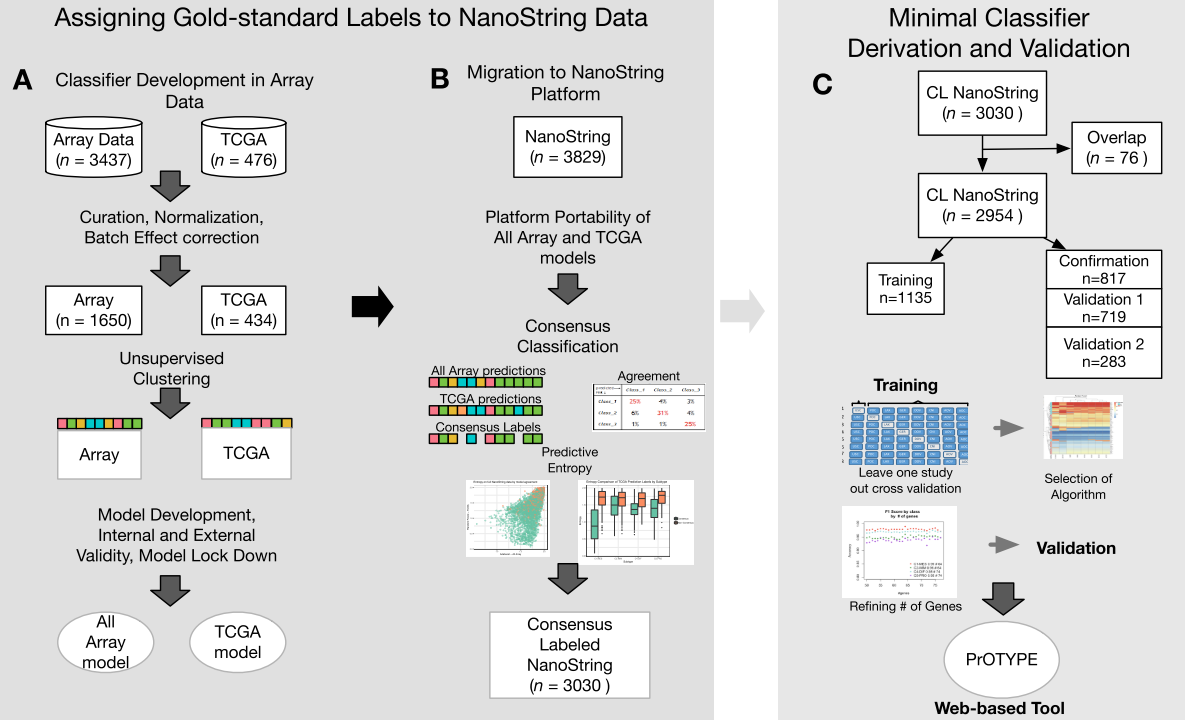
\includegraphics[scale=0.35]{talhouk_figure_1_part.png}
\end{center}
\caption{HGSOC subtype prediction by expression analysis of a focussed gene set and concensus across two independent pipelines.  From \cite{Talhouk2020}.}
\label{fig-talhouk_figure_1_part.png}
\end{figure}


\subsection{Gene expression in HGSOC}

This section focusses on biological and clinical conclusions relating to gene expression in HGSOC and mentions analysis techniques only in passing.

Obesity is known to negatively impact prognosis in ovarian cancer \cite{Cuello2018}, \cite{Au-Yeung2014}.  Cuello \etal\ \cite{Cuello2018} used NMF based clustering on mRNA microarrays and reverse-phase protein arrays to demonstrate an association between cancer driver genes and obesity related genes.

Wang \etal\ \cite{Wang2017c} also use NMF clustering to identify five subtypes of HGSOC informative of outcomes: 1:mesenchymal, 2:immunoreactive, 3:proliferative, 4:differentiated and 5:anti-mesenchymal.  Subtypes 2, 5 are found to be associated with longer survival.

Mairinger \etal\ screened 770 immune related genes to identify 11 differentially expressed genes associated with response to platinum treatment.  They find that expression of HS11B1, DNBT1, CKLF, NUP107. CCL18, LY96, ATG7, SLAMF7, CXCL9 is associated with long survival, while IKBKG and SDHA with short survival.

BRCA1 inactivation is known to cause chromosomal instability in many cancers.  Pradhan \etal\ \cite{Pradhan2010} investigated the role of BRCA1 in HGSOC by copy number and expression analysis, finding surprisingly that inactivation has no relationship with gross genomic alteration.  They leave open the question whether DNA repair by PARP plays a role.   The relationship between BRCA1/2 and DNA repair -- specifically homologous repair deficiency (HRD) -- is picked up by Ewing \etal \cite{Ewing2020}.  They study the complex interplay of single nucleotide variants and large structural variants as they impact BRCA1/2 disruption and thence HRD.  This work suggests that when BRCA1/2 loss is detected in HGSOC patients, there may be a clinical role for PARP inhibitors, since this would prevent error-prone non-homologous repair by PARP, and so selectively kill BRCA1/2 disrupted cells.

Note that several of the studies reviewed here use data from the Australian Ovarian Cancer Study (AOCS): \cite{Winterhoff2016,Patch2015,Ewing2020,Zhang2018,Cuello2018,Au-Yeung2014}.

Stratification of HGSOC by immunohistochemistry is addresses Kamble \etal. \cite{Kamble2019}.  They identify a panel of six biomarkers -- TCF21, E-cadherin, PARP1, Slug and AnnexinA2.   These markers allow stratification into categories including Mesenchymal-to-epithelial transition, Homologous recombination repair and Epithelial-to-mesenchymal transition.  This, they argue, will allow selection of class-specific inhibitor drugs such as Olaparib and Rucaparib.

The platinum based drug Cisplatin is a key treatment in ovarian cancer, yet tumours often develop resistance, possibly related to the host's immune response.  Understanding and predicting such resistance is therefore of clinical importance and is addressed by Maringer \etal\ \cite{Mairinger2019} through expression analysis using the NanoString platform with a panel of 770 immune related genes.   They find the following to be significantly related to platinum resistance: KLRC1, TCF7, CD274, HSD11B1, COLEC12, PDGFC, FCF1, BMI1, TNFRSF9, ATG10, EWSR1.

\subsection{Research Questions}
\begin{enumerate}
\item
Which are the influential genes in HGSOC according
to expression data? Do these confirm published
results?
\item
Which of PCA, ICA and NMF is best suited to this
analysis?
\item
For identified genes, what is the underlying biology of
their action?
\item
Can we discriminate subtypes of HGSOC from
expression data?
\item
Is there value in incorporating somatic and germline
genomic data?
\end{enumerate}

%%%%%%%%%%%%%%% METHODOLOGY %%%%%%%%%%%%%%%%%

\section{Methodology}

\subsection{Outline}

\subsubsection{Datasets}
\begin{enumerate}
\item TCGA, n=274, g=19,601
\item AOCS, n=80, g=19,730
\end{enumerate}

\subsubsection{Method outline}
In outline our method is follows:
\begin{enumerate}
\item
Unsupervised factor extraction by Matrix
factorization methods : NMF, ICA and PCA.
\item
Identification of a consistent gene list between the TCGA and AOCS datasets.
\item
Factor selection for robustness by
k-means clustering and silhouette score
\item
Investigation of biological significance of determined factors by gene enrichment analysis against the Gene Ontology (GO) and Kyoto Encyclopedia of Genes and Genomes (KEGG).
\item
Survival analysis on TCGA to identify key predictive factors
\item
Transfer of identified factors to the AOCS dataset by matrix psuedo-inverse to validate efficacy of identified features.
\item
Revisit enrichment analysis for most significant factors to study biological significance.
\end{enumerate}

\subsubsection{Tools}
\begin{itemize}
\item Python 3.6
\item Numpy for high performance matrix manipulation
\item Pandas for data frame handing
\item Matplotlib for plotting
\item Scikit-learn for matrix factorization and k-means clustering
\item GOATOOLS package for gene enrichment analysis against GO
\item Lifelines package for survival analysis.
\end{itemize}

A full list of software and libraries used, with versions, is given in appendix \ref{sec-software-versions}

\subsection{Data normalization and quality control}

Expression data for the AOCS and TCGA datasets was received for this project in a normalised matrix format.  The full pre-processing pipeline is described in \ref{Ewing2020}, in brief using the DESeq2 package with normalization by variance stabilizing transformation.   

\subsection{Gene set intersection}

In order to allow factorizations found in the TCGA dataset dataset to be applied to the AOCS dataset it is necessary (or at least convenient) to synchronize the set of genes over which the expression matrices are defined.   As provided to this project, the TCGA and AOCS datasets cover 19,610 and 19,730 genes respectively, 19,566 or which common to both (according to ENSG encodings).  Thus, both datasets were pruned to the 19,566 intersection set and ordered consistently.

\subsection{Matrix factorization computation}
One of the aims of this work is to compare the efficacy of three dimensionality reduction methods -- NMF, ICA and PCA -- as explained in the introduction.   The three methods have different properties and notational conventions, but to simplify the discussion here we adopt $X \approx W H$ for all three methods, where $X$ is the (genes, patients) expression matrix  $W$ is the (genes, factors) metagenes matrix and $H$ is the (factors, patients) metasamples matrix.   Please refer back to section \ref{sec-matrix-factorization-intro} for further explanation.

Some of the key algorithm hyper parameters of each method were investigated and tuned with respect to reconstruction accuracy, specifically the root-mean square (RMS) difference between $X$ and $WH$. The following parameters were explored in each case:
\begin{description}
\item[NMF:] Parameters {\tt max\_iter} (algorithm iterations) and {\tt tol} (tolerance of convergence) were optimised for good accuracy and acceptable execution time.  Other parameters of interest are {\tt alpha} (multipluer for regulation term) and {\tt l1\_ratio} (multiplier for L1 regularization, when {\tt alpha} $> 0$).  L1 regularization  favours elements being precisely zero, whereas L2 regularization will encourage them to be small.  These parameters have not been explored in this project, and the default {\tt alpha = 0} (no regularization) was used.
\item[ICA:]  Parameters {\tt max\_iter} and {\tt tol} we investigated as for NMF above.  Additionally, options for the entropy functional which forms the basis of the optimiziation were investigated.
\item[PCA:] This is in principle a deterministic algorithm based on eigenvector decomposition.  However, {\tt sklearn.decomposition.PCA} uses a more efficient 'randomized' algorithm when the given matrix is larger than 500 in both dimensions.  Thus in our use case PCA is seen to have stochastic behaviour.

\end{description}

\subsection{Factor selection by cluster coherence}

As outlined in the discussion, deciding the number of components (metagenes) to extract is key.  Taking more components results in more accurate representation of the observed expression matrix and provides more avenues to explore the underlying biology.  However, it is important that the metagenes are \emph{stable}, that is likely to have reliable meaning when transfered to other datasets.   There are two sources of variation or instability to consider.

NMF and ICA are inherently stochastic algorithms, sensitive to their starting state, so repeated runs give different results.

A second and more fundamental source of variation of relevance to all three factorization methods is \emph{sampling error}.   Our factorizations are based on a small (N=80 or N=374) sample of patients drawn from the population of HGSOC patients; our particular datasets are just two examples of many different `draws' which could have been made.  

\emph{Bootstrap sampling} (also know as \emph{Monte Carlo} simulation) is a common method of empirically propagating the consequence of sampling error when the distribution or processing operations are difficult to model mathematically.   This is implemented by performing factorizations multiple times, at each iterations choosing N samples from the N available \emph{with replacement}.   For this work 50 repeats were performed, being a compromise between achieving an adequate simulation without overly burdensome computation time.  The overall process is summarised as pseudocode in figure \ref{fig-clustering-psuedocode}.  

Each of the three factorizer methods is evaluated for rank $k$ between 2 and 10.  In each case, 50 iterations of factorization are performed on bootstrap samples, generating $50 k$ 19,566 dimensioned metagenes.   t-SNE plots \ref{tsne-reference} visualise these high-dimensioned metagenes in a 2-D view.   If sampling and algorithm initialisation error are modest then we expect to see $k$ clusters of points.   To avoid lengthy computation in the t-SNE clustering, the metagenes are first reduced to $r=20$ dimensions by PCA; brief experiments showed that this reduction had negligible effect on the t-SNE visualisation for $r \geq 10$.

In order to obtain median estimates of the $k$ metagenes from the $50 k$ which were generated, k-means clustering was performed in the PCA reduced (20 dimension) space, delivering $k$ sets of points.  These were referenced back to the original 19,566 dimensioned metagenes and the per-dimension median calculated.  These $k$ median metagenes were saved a file named for the specific factorizer and rank $k$.  

The k-means clustering further allowed for a quantitative assessment of cluster coherence for the particular choice of factorizer and rank, via the \emph{silhouette score}.  In brief, this is a measure of how close (by Euclidean distance) each point in a cluster is to other points in the cluster versus points \emph{not} in the same cluster.  See 
% \href{https://en.wikipedia.org/wiki/Silhouette_(clustering)}{Wikipedia: Silouette (clustering)}.  
The score is in the range -1 to +1, with 0 implying random scatter and 1 implying all points of a cluster overlay.

The t-SNE plots and silhouette scores were assessed visually (see figures \ref{fig-first-cluster-result} to \ref{fig-last-custer-result} to decide, for each of the three factorizers, the highest rank with good cluster coherence, those median metagenes to take forward to gene enrichment and survival analysis.  

Initial investigation on the N=80 AOCS dataset showed very poor coherence, even for k=2.   Thus it was decided compute and select metagenes only from the N=374 TCGA dataset.   We refer to those selected ranks as $K_{\mbox{\tiny NMF}}$ etc., thus yielding $K_{\mbox{\tiny NMF}} + K_{\mbox{\tiny ICA}} + K_{\mbox{\tiny PCA}}$ metagenes in total.

\begin{figure}
\begin{center}
\begin{Verbatim}[baselinestretch=1, frame=single, rulecolor=\color{blue}, label=Metagene Stability Assessment, fontfamily=courier, fontsize=\small]

 for factorizer in NMF, ICA, PCA:
    for k in 2..11:
       Ws = []
       for j in 1..50:
          X = bootstrap sample N from N
          W, H = factorizer(X, rank=k, seed=j)
          append W to Ws
   	     
          # Ws is a list of 50*k metagenes, each of length 19,566
          # Pragmatically reduce metagenes to 20 dimensions by PCA
   	  
       Ws_reduced = PCA(Ws, rank=20)
       plot t-SNE(Ws_reduced)
       clustering = k-means clustering(Ws_reduced, n_clusters=k)
       score[factorizer, k] = silhouette score(clustering)	  
       median_metagenes = calculate medians for k clusters of metagenes
       save median_metagenes to file by factorizer and k
       for each factorizer 
          plot score vs k
      
\end{Verbatim}
\end{center}
\caption{Pseudocode for generating median metagenes and assessing there stability to random algorithm initialization and sampling error.}
\label{fig-clustering-psuedocode}
\end{figure}
	   	  
\subsection{Gene enrichment analysis}

\subsection{Survival analysis}

Survival analysis was performed to investigate whether the selected metagene factors correlated with patient survival.  Overall  survival (OS) data is available for both the TCGA and AOCS datsets.  Additionally, progression free survival (PFS) data is available for AOCS.   As discussed in section \ref{sec-clustering-method}, metagenes were obtained by factorization on the TCGA dataset only.  Application to TCGA (for OS) thus represents an in-sample test, while application to AOCS (for OS and PFS) is a more exacting out-of-sample test. There are thus three analyses to consider: 1) TCGA$\rightarrow$TCGA (OS), 2) TCGA$\rightarrow$OACS (OS) and 3) TCGA$\rightarrow$OACS (PFS).

Analysis was performed using the Python {\tt Lifelines} package \cite{Davidson-Pilon2020}.  Metasamples ($H$ matrices) were calculated from the metagenes and expression matrix as explained in section \ref{sec-transfer-to-novel} below.  Metasample values were binariased to 0, 1 by thresholding at the median value.   Kaplan-Meier plots were made in respect of derived metasample for each of the three analysis -- making $11 \times 3$ plots each with two survival curves (with 95\% confidence intervals).  A hazard ratio (HR)
\comment{Do I need to explain the definition and meaning of HR?} 
was calculated for each plot by fitting Cox's proportional hazards model with p-value relating to the hypothesis that HR is significantly different to 1.0.

\subsection{Transfer of learned factors to novel a dataset}
\label{sec-transfer-to-novel}

\newcommand{\trainset}{\mathcal{T}}
\newcommand{\validset}{\mathcal{V}}

Rank $k$ matrix factorization on the training dataset $\trainset$ (specifically the TCGA dataset) results in:
\begin{equation}
 X_\trainset \approx W_\trainset H_\trainset
\end{equation}
where $X_\trainset$ is the expression matrix of shape $(g_\trainset, n_\trainset)$, with $g_\trainset$ the number genes and $n_\trainset$ the number of patients. $W_\trainset$ is the metagene matrix of shape $(g_\trainset, k)$ and $H_t$ is the metasamples matrix of shape $(k, n_\trainset)$.

We wish to apply the factorization learned on $\trainset$ to a novel dataset $\validset$ (specifically the AOCS dataset) of shape $(g_\validset, n_\validset)$. Importantly, $n_\validset = 1$ reflects the application of these methods to a single patient in a clinical setting.  To apply the learned factorization we need to find $H_\validset$ as in the factorization
\begin{equation}
	X_\validset \approx W_\validset H_\validset
\end{equation}
In both the experimental and clinical situation we are given $X_\validset$ but not $W_\validset$ and require to find $H_\validset$.  We \emph{cannot} simply perform the matrix factorization on dataset $\validset$ since $n_\validset$ may be small, or even a single patient.   However, if patients in datasets $\trainset$ and $\validset$ are drawn from the same population (ovarian cancer patients), then $X_\trainset$ and $X_\validset$ can be expected to have similar distributions w.r.t to their columns, and thus $W_\trainset$ and $W_\validset$ can be expected to be equivalent within sampling error.  This only makes sense if the two expression matrices $X_\trainset$ and $X_\validset$ are defined over the \emph{same list of genes}, so that $g_\trainset = g_\validset = g$, in which case $W_\trainset$ and $W_\validset$ have the same shape of $(g, k)$.   

We thus need to solve for $H_\validset$ in
\begin{equation}
	X_\validset  \approx  W_\trainset H_\validset \label{eq_Xv_WtHv}
\end{equation}

This can be solved by the method of least squares.  In the case that the original factorization was by NMF, we use non-negative least square regression (NNLS):
\begin{equation}
	H_\validset = \mbox{argmin}_{H\geq 0}{\lvert W_\trainset H - X_\validset \rvert}_2
	\label{eq_Hv_WdtXv}
\end{equation}
where ${\lvert \mathbf{\cdot} \rvert}_2$ indicates Euclidean distance or L2-norm.
The Python library function {\tt scipy.optimize.nnls} is used.

For ICA and PCA we use ordinary least square regression, formulated above by dropping the $H\geq 0$ constraint, using {\tt sklearn.linear\_model.LinearRegression}.

An internal check on the validity of the statistical assumptions can be made my substituting  $H_\validset$ from (\ref{eq_Hv_WdtXv}) into (\ref{eq_Xv_WtHv}) and assessing the accuracy of the approximation by RMS difference.

The end result of the analysis the $H_\validset$ matrix of shape $(k, n_\validset)$, thus delivering for dataset in our $\validset$ a feature vector of length $k$ -- a small number typically less than a dozen.

Since in this work we wish to evaluate the efficacy of the three factorization methods -- NMF, ICA and PCA -- we in fact take forward three different $H$ matrices, having not necessarily the same rank $k$.

\subsection{Survival analysis on novel dataset}

\subsection{Study of biological significance of predictive factors}

\subsection{Codebase}

The described method was implemented in Python, except for the KEGG gene enrichment analysis which was implemented in R.  All code is available in a github repository: \url{https://github.com/ipoole/HgsocTromics}.  Good software engineering practice has been followed, with an object-oriented design, frequent commits and unit testing.  Unit tests are based on tiny expression matrices, just 100 genes by 10 patients, so that the whole test suite executes in around 10 seconds.  These tests are particularly valuable when re-factoring code by providing a rapid means of detecting errors.  All plots are generated in vector graphics pdf format to ensure smooth scaling to any resolution. 



%%%%%%%%%%% RESULTS %%%%%%%%%%%%%

\section{Results}

Results of the above described methodology are explained and presented here.   Deeper interpretation and discussion is deferred to the following section.  Throughout, consistent colours of \textcolor{blue}{blue}, \textcolor{orange}{orange} and \textcolor{green}{green} are used for results relating to NMF, ICA and PCA respectively.

\subsection{Investigation of optimal parameters}

\subsection{Cluster coherence analysis results}

Figure \ref{fig-AOCS-ica-fixed-vs-bootstrap} demonstrates that resampling error on a small N=80 dataset makes metagene extraction highly unstable, effectively un-usable.  For brevity only results for ICA are shown, but a very similar effect is observable for PCA and NMF.   For this reason it was decided to perform all metagene extraction on the larger N=374 TCGA dataset, in which the impact of sampling error is not so severe -- see figure \ref{fig-TCGA-ica-fixed-vs-bootstrap}.  

The critical decision of the choosing the facorization rank for each method -- $K_{\mbox{\tiny NMF}}$, $K_{\mbox{\tiny ICA}}$ and $K_{\mbox{\tiny PCA}}$ -- is based on figure \ref{fig-TCGA-all-bootstrap}.   On this bases, considering both the t-SNE plots and silhouette scores, for following choices were made:
$K_{\mbox{\tiny NMF}}  =  3,
K_{\mbox{\tiny ICA}}  =  5,
K_{\mbox{\tiny PCA}}  =  3$.

The rationalle for these choices is that, firstly $k>2$ is desirable to have sufficient information to work with.  NMF cluster coherence seems to deteriorate after $k=3$.   Looking at the graph of silhouette scores, ICA appears to have a sweet spot at $k=5$.  For PCA, $k = 3$ or $4$ both seem reasonable, $k=3$ is safe.

\def\S{0.4}
\begin{figure}
\begin{center}
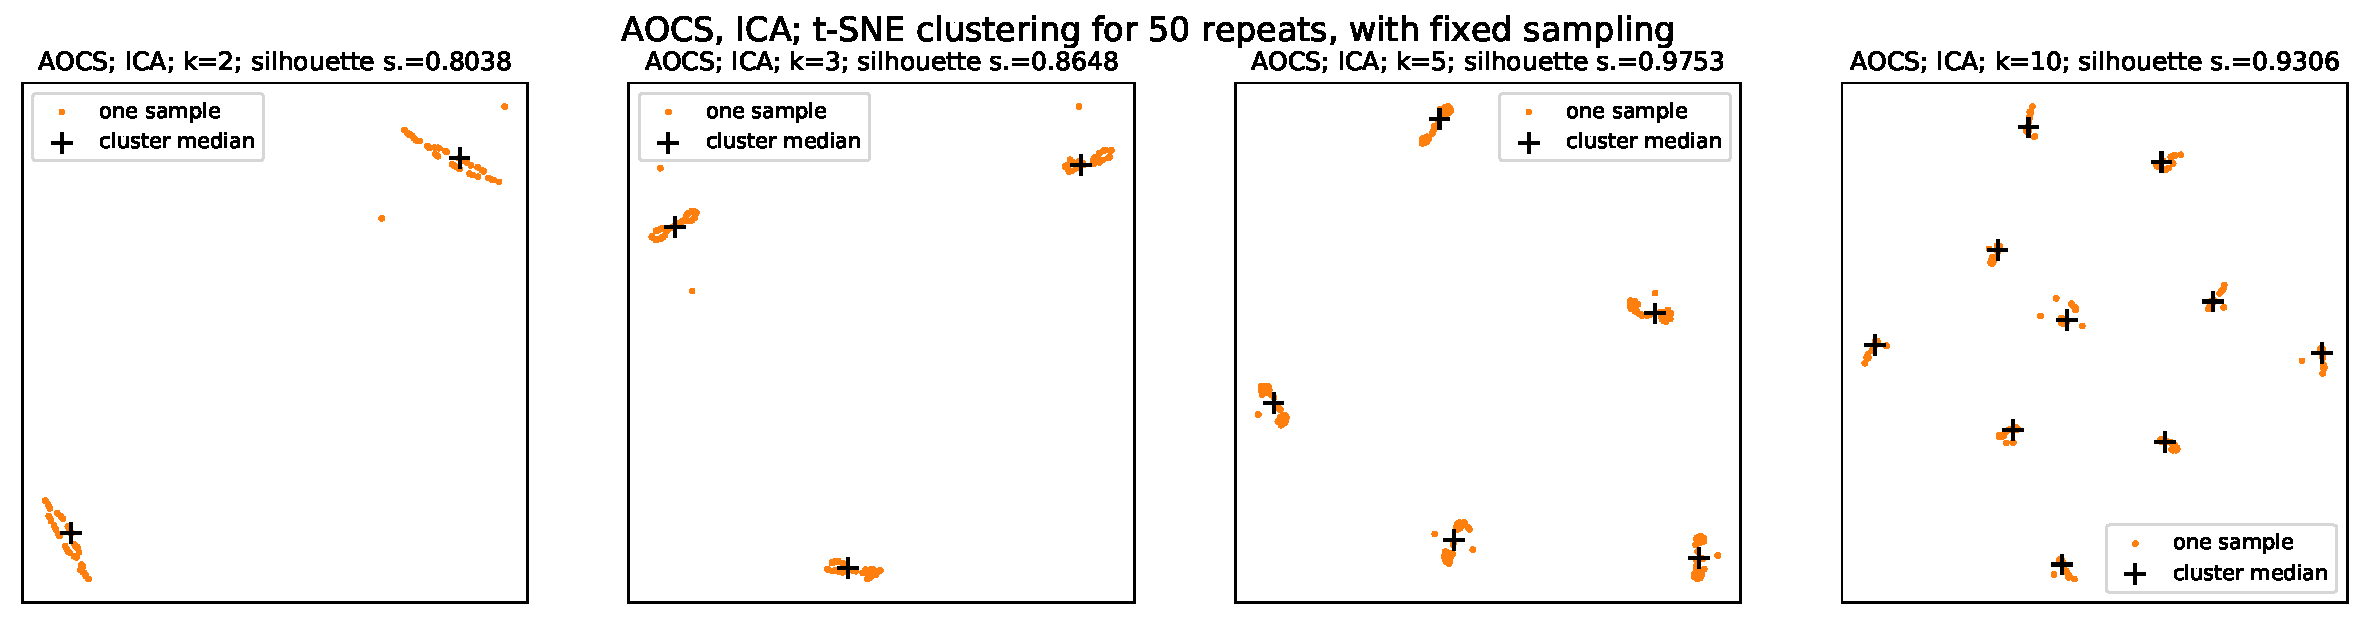
\includegraphics[scale=\S]{\plotspath{AOCS_Protein/FactorClustering/multiple_single_factors_scatter_AOCS_ICA_2_3_5_10_fixed.pdf}} \\
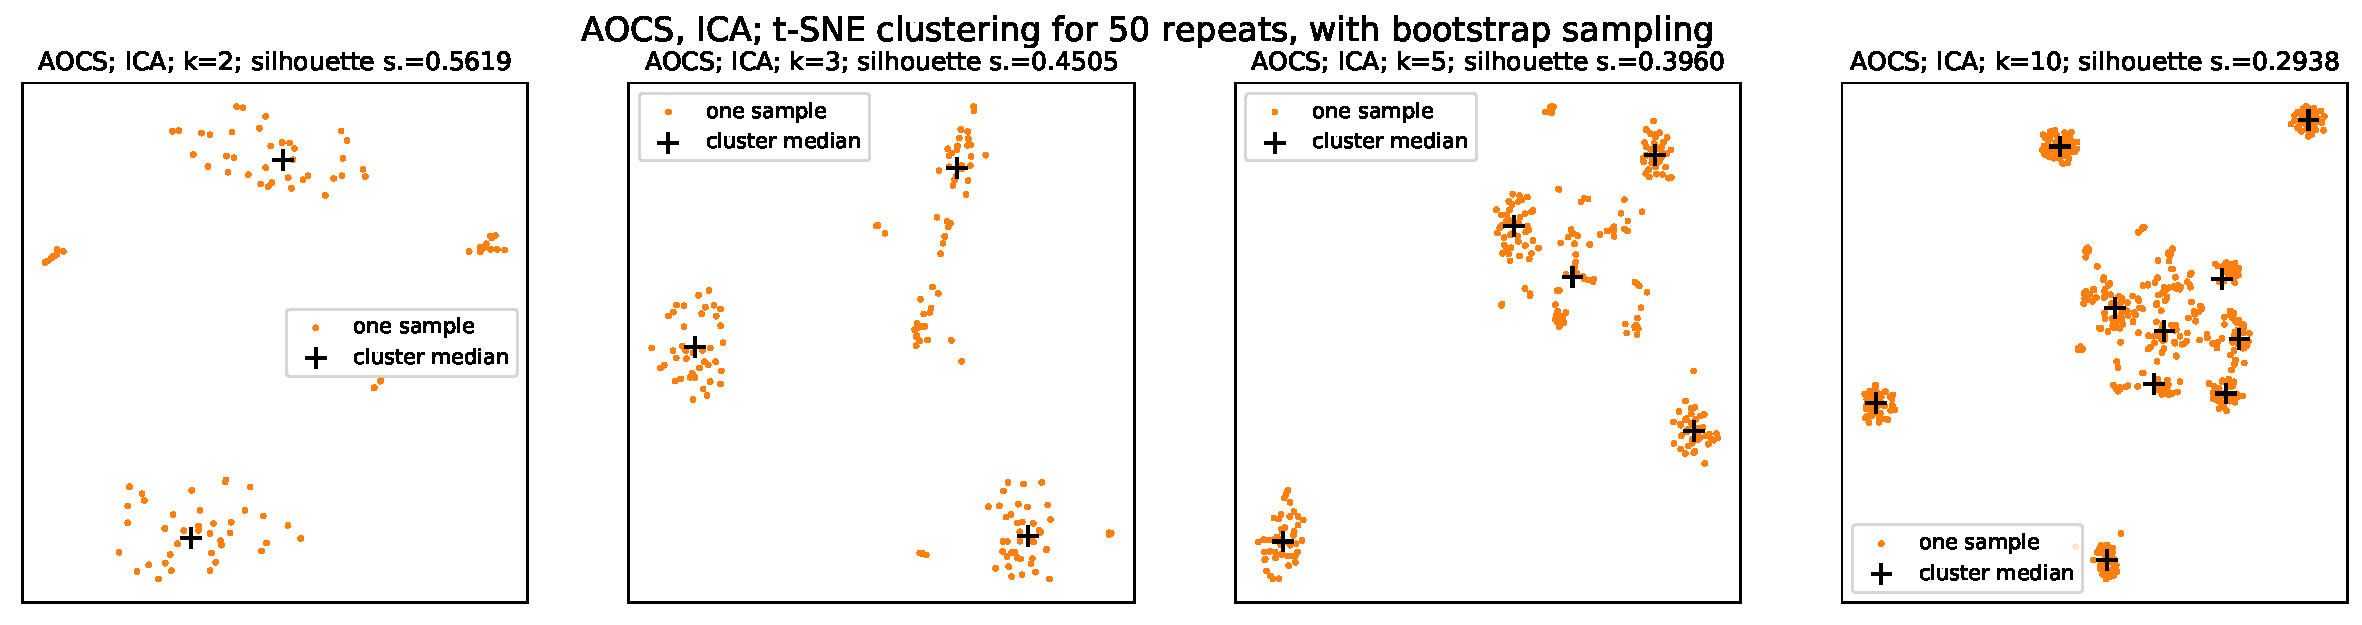
\includegraphics[scale=\S]{\plotspath{AOCS_Protein/FactorClustering/multiple_single_factors_scatter_AOCS_ICA_2_3_5_10_bootstrap.pdf}}\\
\caption{Clustering of metagenes from ICA facorizations on the N=80 AOCS dataset, comparing \emph{fixed} sampling (top row) with \emph{bootstrap} sampling (bottom row) for a selection of factorization ranks.  With sampling error excluded, clusters appear reasonably coherent, but when sampling error is modelled by bootstrap sampling then we see the factorizations become much less stable.}
\label{fig-AOCS-ica-fixed-vs-bootstrap}
\end{center}
\end{figure}

\begin{figure}
\begin{center}
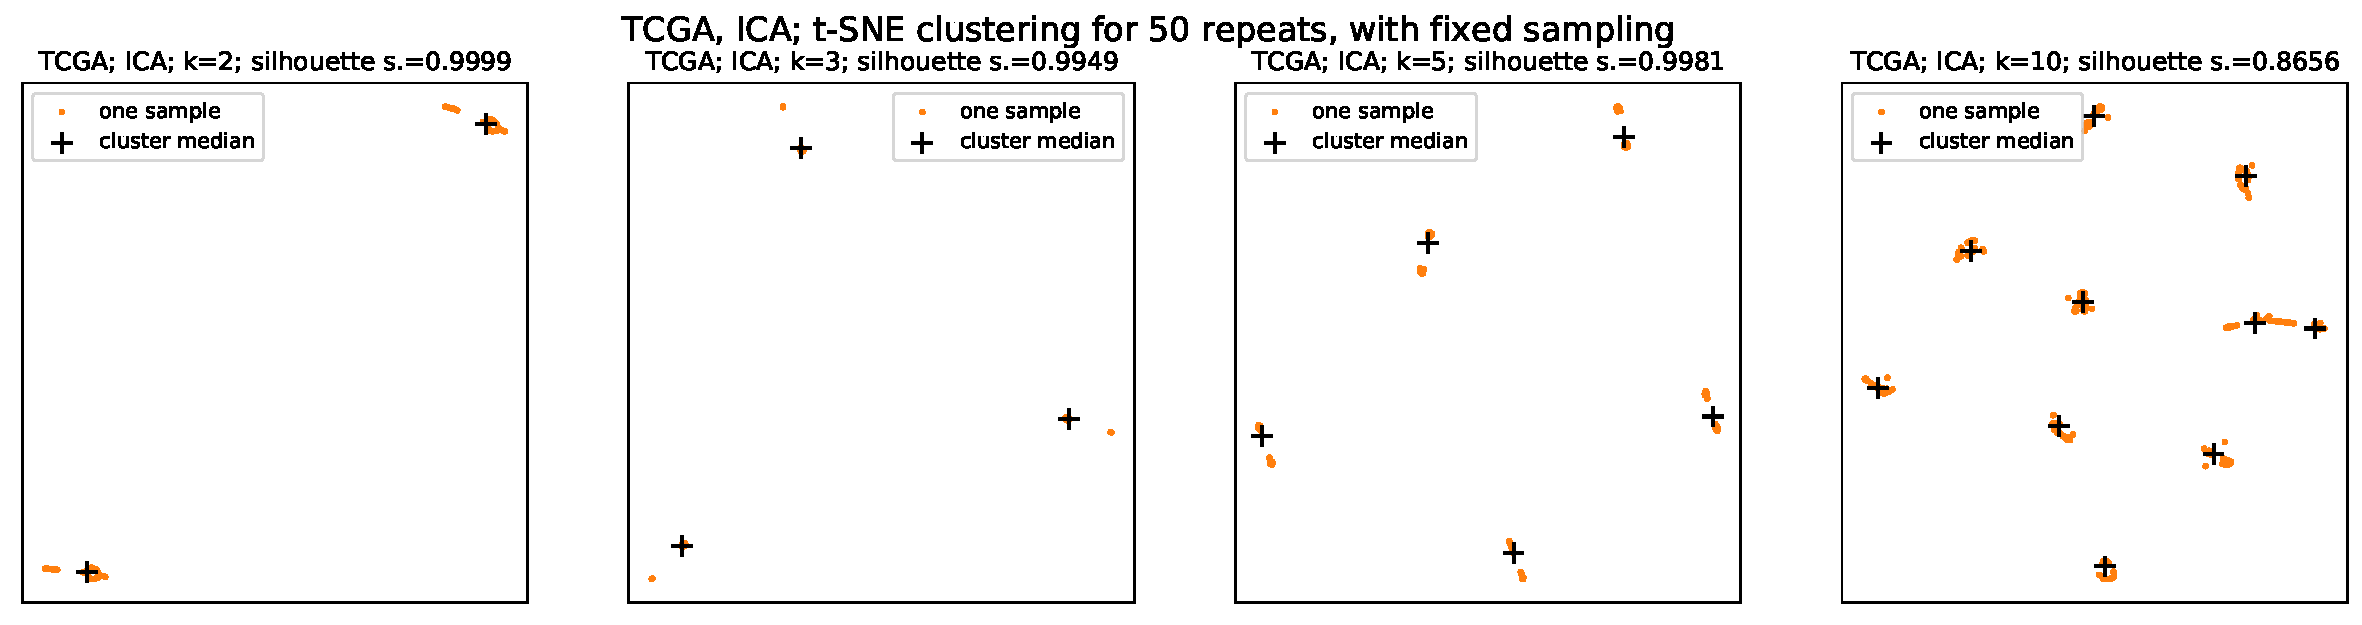
\includegraphics[scale=\S]{\plotspath{TCGA_OV_VST/FactorClustering/multiple_single_factors_scatter_TCGA_ICA_2_3_5_10_fixed.pdf}} 
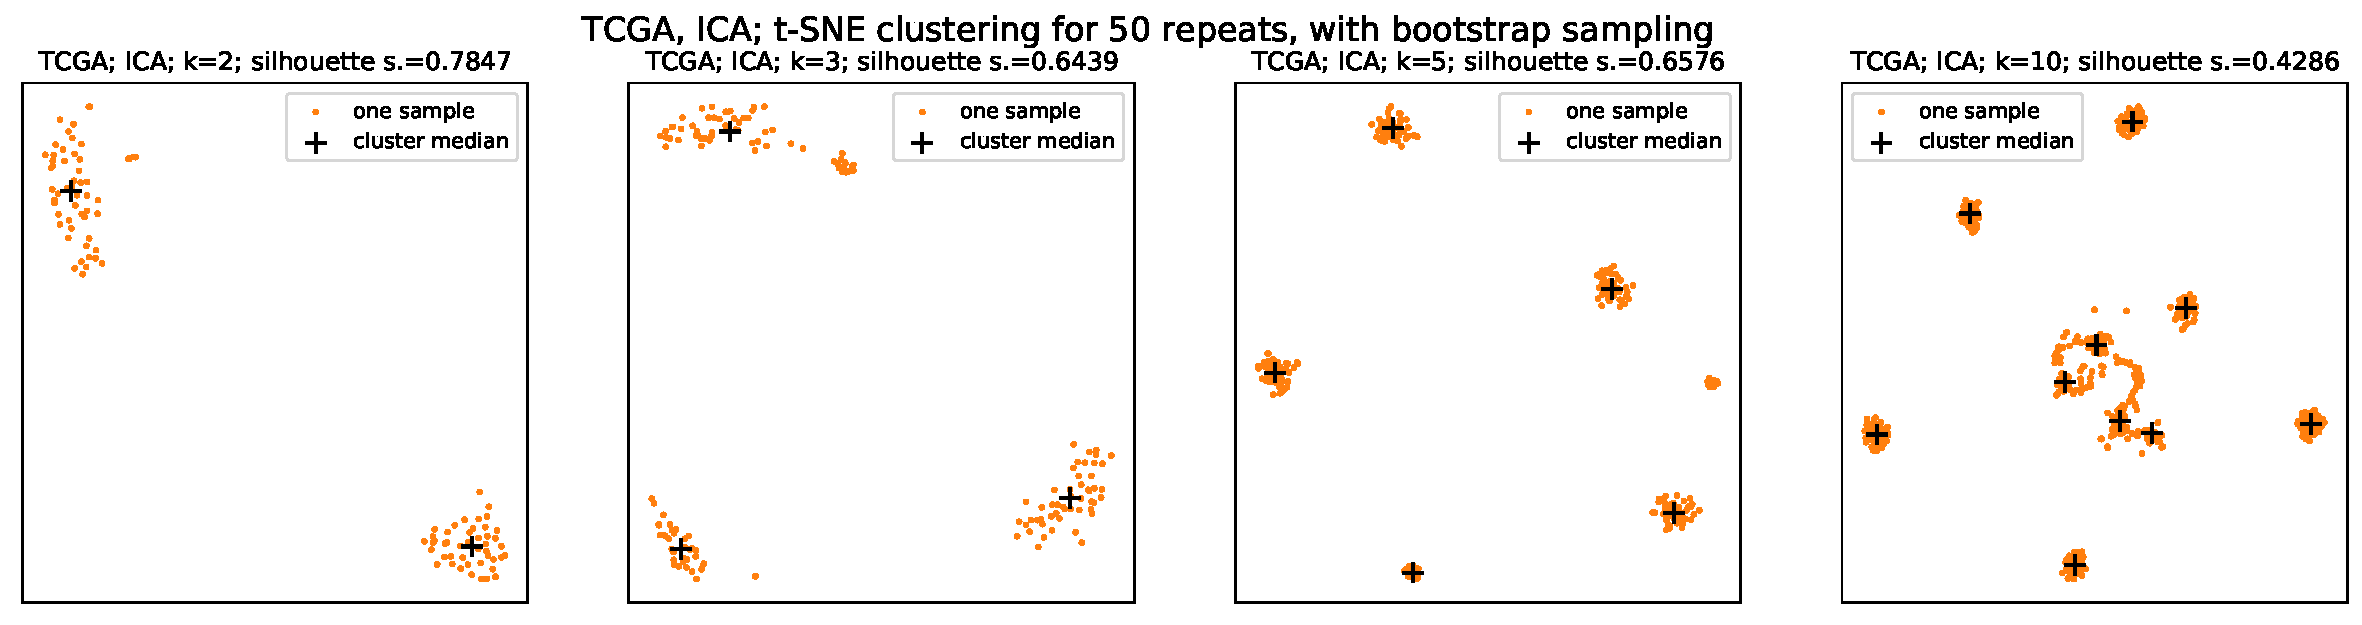
\includegraphics[scale=\S]{\plotspath{TCGA_OV_VST/FactorClustering/multiple_single_factors_scatter_TCGA_ICA_2_3_5_10_bootstrap.pdf}}
\caption{Clustering of metagenes from ICA facorizations on the N=374 TCGA dataset, again comparing fixed and bootstrap sampling.  In this larger dataset, sampling error (bottom row) is not so severe; compare with figure \ref{fig-AOCS-nmf-fixed-vs-bootstrap}}
\label{fig-TCGA-ica-fixed-vs-bootstrap}
\end{center}
\end{figure}

\begin{figure}
\begin{center}
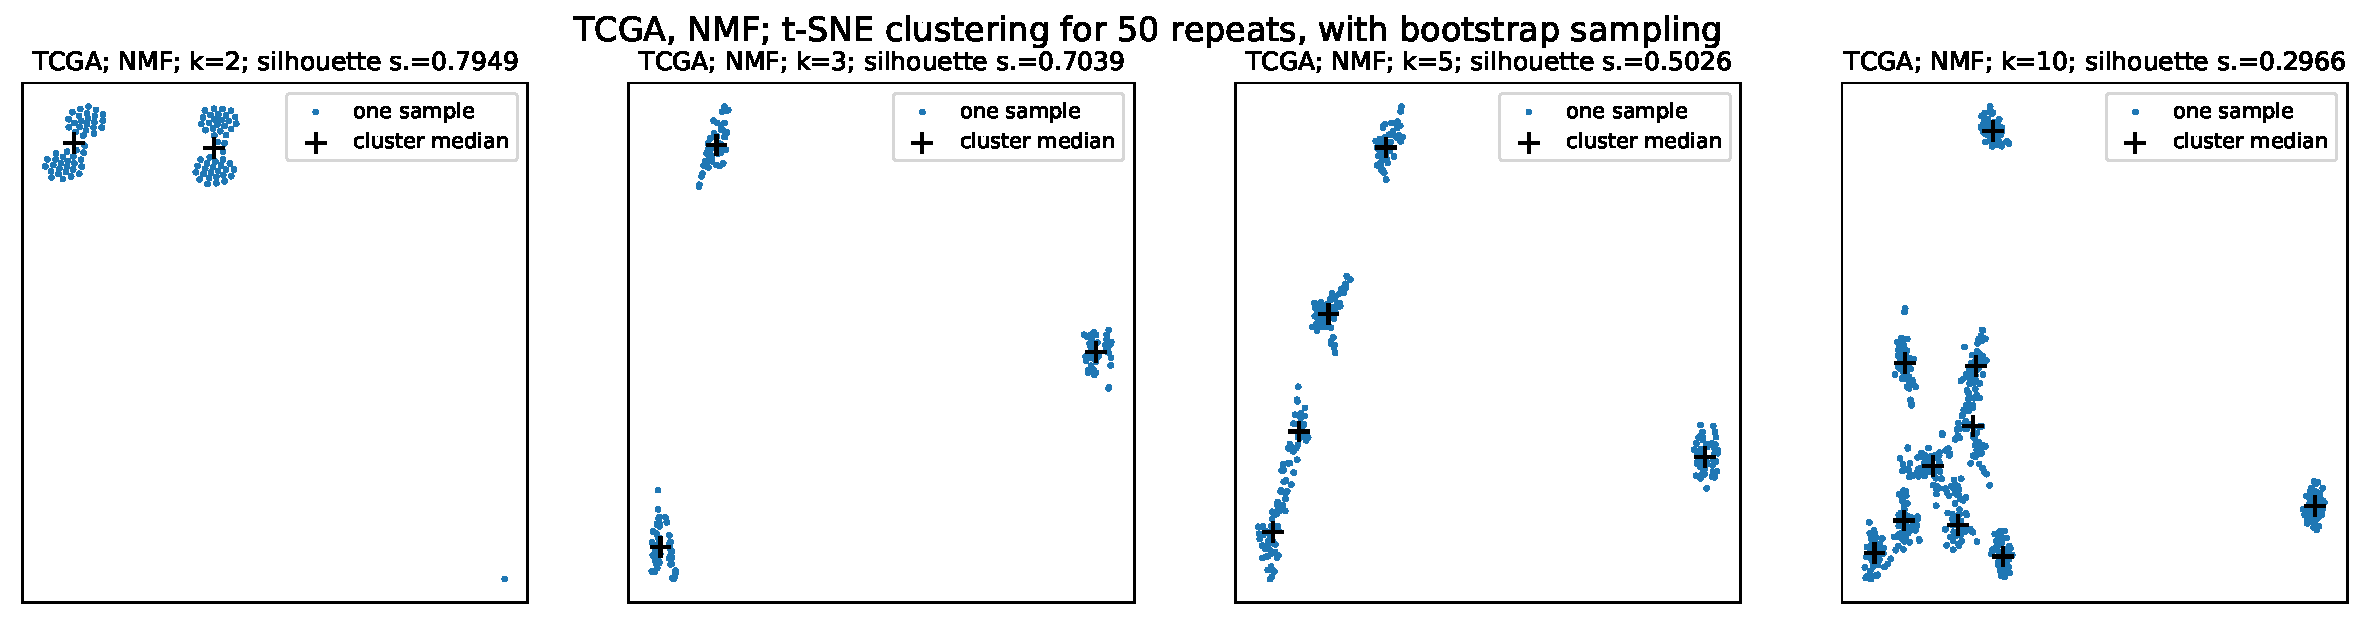
\includegraphics[scale=\S]{\plotspath{TCGA_OV_VST/FactorClustering/multiple_single_factors_scatter_TCGA_NMF_2_3_5_10_bootstrap.pdf}} \\
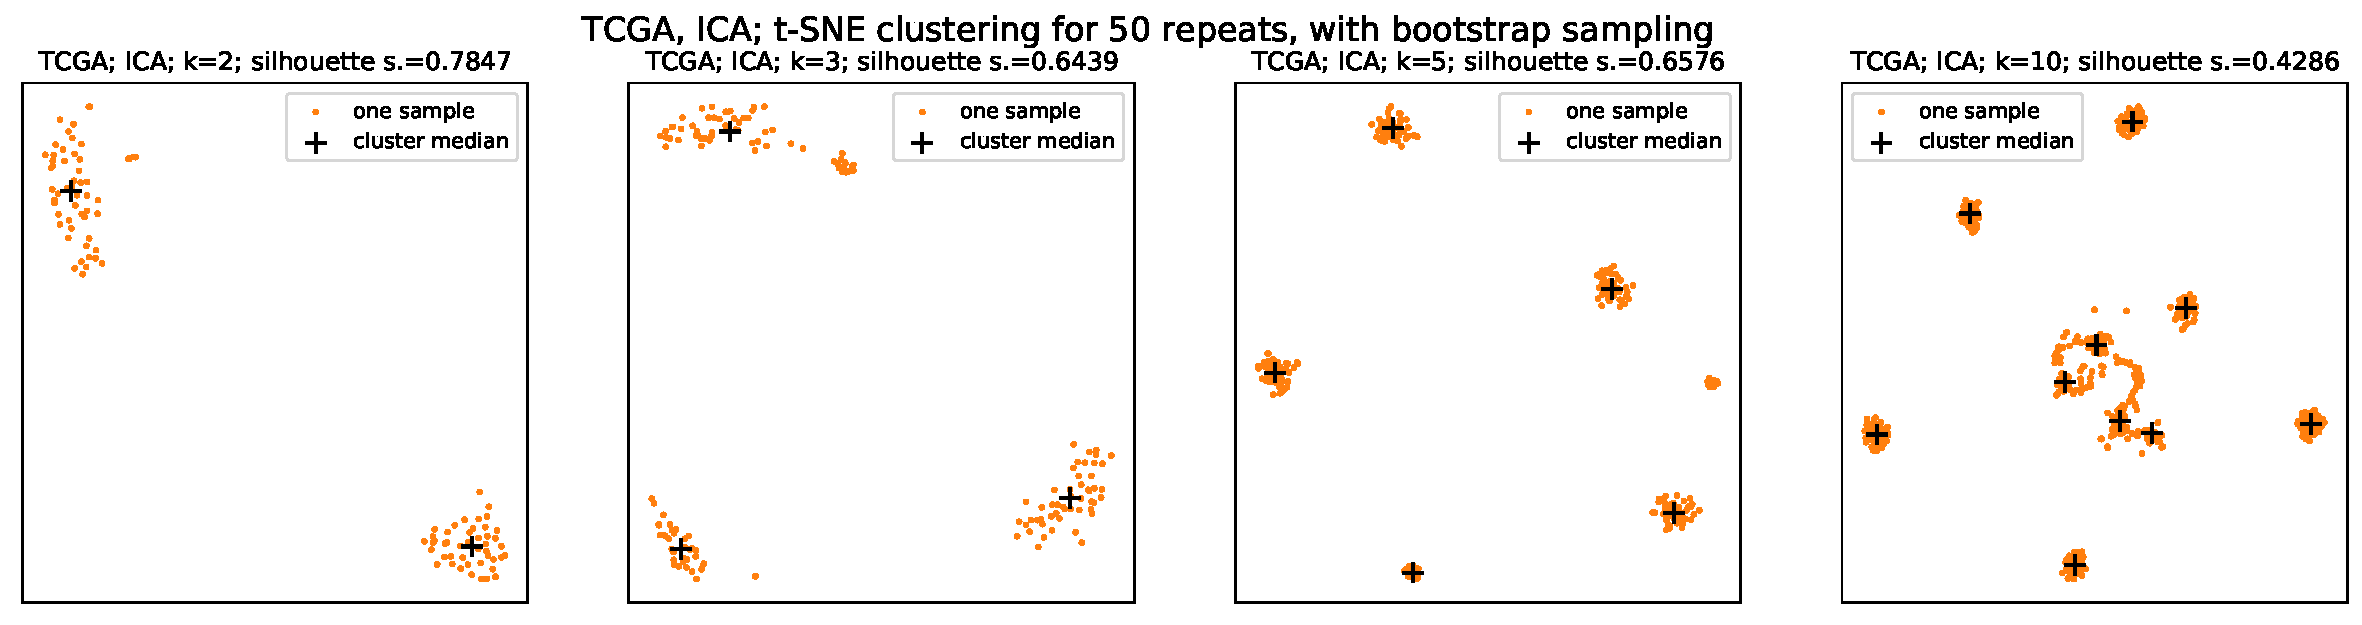
\includegraphics[scale=\S]{\plotspath{TCGA_OV_VST/FactorClustering/multiple_single_factors_scatter_TCGA_ICA_2_3_5_10_bootstrap.pdf}} \\
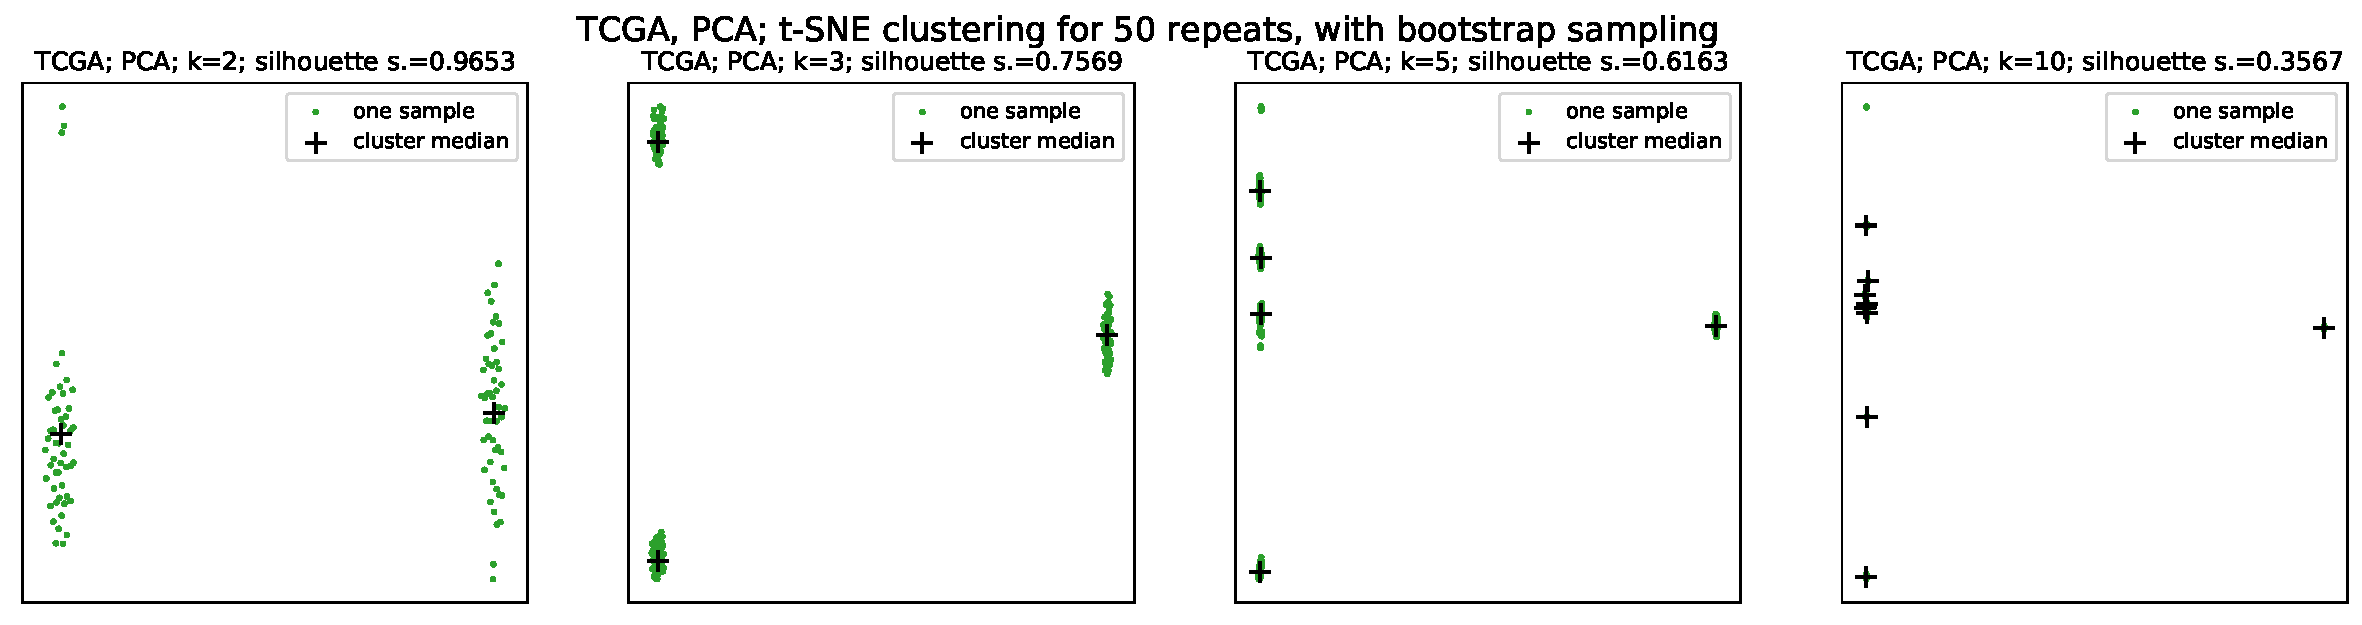
\includegraphics[scale=\S]{\plotspath{TCGA_OV_VST/FactorClustering/multiple_single_factors_scatter_TCGA_PCA_2_3_5_10_bootstrap.pdf}} \\
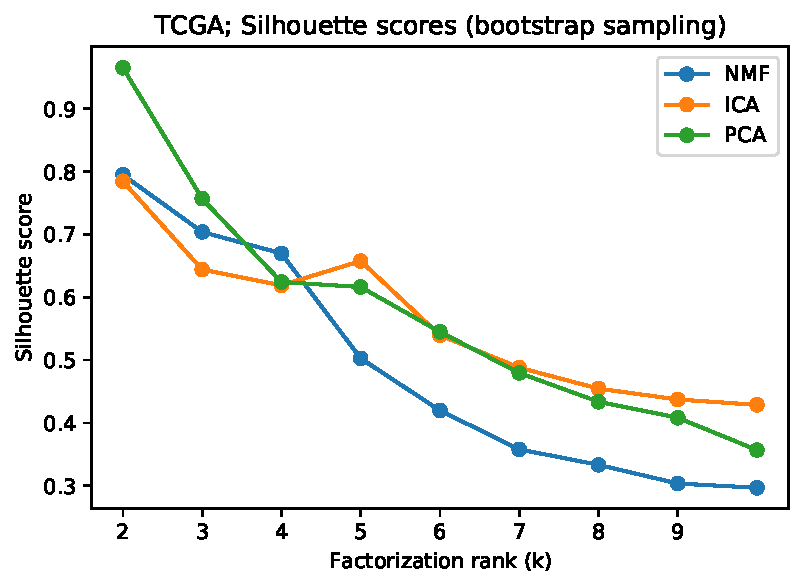
\includegraphics[scale=0.45]{\plotspath{/TCGA_OV_VST/FactorClustering/silhouette_plots_TCGA_2_3_4_5_6_7_8_9_10_bootstrap.pdf}} 
\caption{Metagene clustering for all three methods applied to the N=374 TCGA dataset with bootstrap sampling, over a range of factorization ranks.  The silhoutte scores are also plotted (bottom).  It is on the basis of this figure that the factorization ranks for each method were selected.}
\label{fig-TCGA-all-bootstrap}
\end{center}
\end{figure}


\subsection{Survival analysis results}

\begin{figure}
\begin{center}
\includegraphics[scale=0.5]{\plotspath{SurvivalAnalysis/multiple_kaplan_meier_os_TCGA_TCGA.pdf}} 
\caption{Kaplan-Meier plots for each metasample component, stratified at the median value, for TCGA $\rightarrow$ TCGA for overall survival (OS) case.  Hazard ratio and p-value is shown for each case.  The final plot (bottom right) is unstratified overall survival}
\label{fig-kaplan-meier-os-TCGA-TCGA}
\end{center}
\end{figure}


\begin{figure}
\begin{center}
\includegraphics[scale=0.5]{\plotspath{SurvivalAnalysis/multiple_kaplan_meier_os_TCGA_AOCS.pdf}} 
\caption{Kaplan-Meier plots for TCGA $\rightarrow$ TCGA for overall survival (OS) case.}
\label{fig-kaplan-meier-os-TCGA-OACS}
\end{center}
\end{figure}


\begin{figure}
\begin{center}
\includegraphics[scale=0.5]{\plotspath{SurvivalAnalysis/multiple_kaplan_meier_pfs_TCGA_AOCS.pdf}} 
\caption{Kaplan-Meier for TCGA $\rightarrow$ TCGA for progression free survival (PFS) case.  }
\label{fig-kaplan-meier-pfs-TCGA-OACS}
\end{center}
\end{figure}


\begin{figure}
\begin{center}
\includegraphics[scale=0.5]{\plotspath{/SurvivalAnalysis/survival_summary_barplots_NMF.pdf}} \\
\includegraphics[scale=0.5]{\plotspath{/SurvivalAnalysis/survival_summary_barplots_ICA.pdf}} \\
\includegraphics[scale=0.5]{\plotspath{/SurvivalAnalysis/survival_summary_barplots_PCA.pdf}} \\
\caption{Visual summary of survival analysis as applied to TCGA(OS), AOCS(OS) and AOCS(PFS).  Plots are divided by factorization method.  Bar heights show $\log_2(HR)$ with p-value also shown.  For a component to have robust correlation with survival we expect all three of the analysis bars to pass a significance threshold {\em and} for the $\log{HR}$ to to be {\em in the same sense\/}.  None achieve this.}
\label{fig-summary-survival-plots}
\end{center}
\end{figure}


%\begin{table}
%\begin{center}
%\small
%% \renewcommand{\arraystretch}{0.75}
%\input{/home/ipoole/Documents/gitrepos/HgsocTromics/Plots/SurvivalAnalysis/survival_analysis_table_os_TCGA_TCGA.tex}
%\end{center}
%\caption{Survival analysis (overall survival) for TCGA stratified at the median of each of the selected components}
%\label{tab-survival-os_TCGA_TCGA}
%\end{table}
%
%
%\begin{table}
%\begin{center}
%\small
%% \renewcommand{\arraystretch}{0.75}
%\input{/home/ipoole/Documents/gitrepos/HgsocTromics/Plots/SurvivalAnalysis/survival_analysis_table_os_TCGA_AOCS.tex}
%\end{center}
%\caption{Survival analysis (overall survival) for OACS stratified at the median of each of the selected components}
%\label{tab-survival-os_TCGA_AOCS}
%\end{table}
%
%
%\begin{table}
%\begin{center}
%\small
%% \renewcommand{\arraystretch}{0.75}
%\input{/home/ipoole/Documents/gitrepos/HgsocTromics/Plots/SurvivalAnalysis/survival_analysis_table_pfs_TCGA_AOCS.tex}
%\end{center}
%\caption{Survival analysis (progression free survival) for OACS stratified at the median of each of the selected components}
%\label{tab-survival-hr_pfs_TCGA_AOCS}
%\end{table}


\section{Discussion}
\begin{itemize}
\item Importance of taking account of sampling error.
\item Little correlation with survival time - not surprising.
\end{itemize}

\section{Conclusions}


\bibliography{OvarianCancer}
\bibliographystyle{ieeetr}

\section{Appendices}

\subsection{Software libraries and versions}
\label{sec-software-versions}


\end{document}